\chapter{Practical examples}\label{chap:chap4}

\section{First example}

This first example is taken from Infer.NET's tutorial \cite{InferNET14t}, and we can see
the resulting representation in Figure \ref{fig:firstExample}, which generates the following code:

\begin{lstlisting}
  using System;
  using System.Collections.Generic;
  using System.Text;
  using MicrosoftResearch.Infer.Models;
  using MicrosoftResearch.Infer;

  namespace Examples
  {
  	public class FirstExample
  	{
  		public void Run()
  		{
  			InferenceEngine engine = new InferenceEngine();
  			engine.Algorithm = new ExpectationPropagation();
        Variable<bool> firstCoin;
  			Variable<bool> secondCoin;
  			Variable<bool> bothHeads;

  			firstCoin = Variable.Bernoulli(0.5).Named("firstCoin");
        secondCoin = Variable.Bernoulli(0.5).Named("secondCoin");
        bothHeads = (firstCoin & secondCoin).Named("bothHeads");

        if (!(ie.Algorithm is VariationalMessagePassing)) {
  				Console.WriteLine(String.concat("Probability both coins are heads: ", ie.Infer(bothHeads));
  				bothHeads.ObservedValue = false;
  				Console.WriteLine(String.concat("Probability distribution over firstCoin: ", ie.Infer(firstCoin));
  			} else {
  				Console.WriteLine("This example does not run with Variational Message Passing");
    		}
  	}
  }
\end{lstlisting}

The generated code is fairly similar to one that a human would
write, with the exceptions of string concatenation (in this case it would be more natural
to join the text with the inference result via the plus operator rather than
using String.concat) and variables being declared and set in different lines.

It is our belief that the graphical representation is clearar than its textual
counterpart, mainly because parameters are named (it is clear that 0.5 is the
probability of true when defining a Bernoulli distributions) and due to the use
of colors: red for statements related with
the inference engine, dark yellow for boolean distributions, green for text
and I/O, blue for booleans and control structures and purple for numbers.

\begin{figure}[t]
  \begin{center}
    \leavevmode
    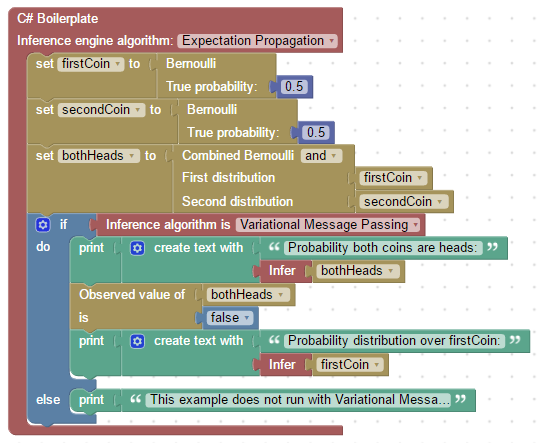
\includegraphics[width=0.86\textwidth]{firstExample}
    \caption{First example of a PP with our Blockly-powered VPE.}
    \label{fig:firstExample}
  \end{center}
\end{figure}

\section{Second and third examples}

\section{Conclusions}
